\section{Summation} \label{append:sum}

\begin{figure}[h!]
\centering
\begin{subfigure}[t]{.475\textwidth}
  \centering
  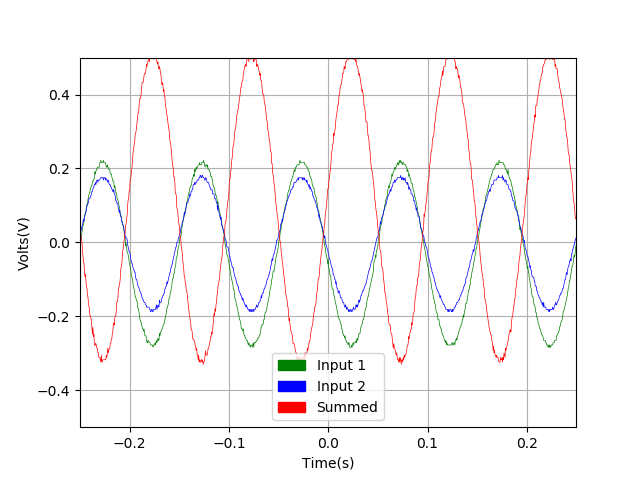
\includegraphics[width=0.95\textwidth, height=0.20\textheight]{figures/Summing/scope_0raw.png}
  \caption{The raw data from the oscilloscope. Inputs (V1, V2) and the Summed Signal (V0)}
 \label{fig:sum_0_og_data}
\end{subfigure}\hfill
\begin{subfigure}[t]{.475\textwidth}
  \centering
  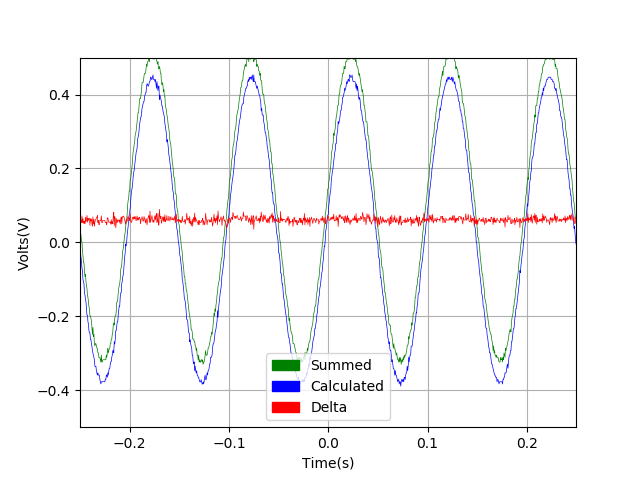
\includegraphics[width=0.95\textwidth, height=0.20\textheight]{figures/Summing/scope_0.png}
  \caption{The summed raw data (V), calculated signal -($v_1 + v_2$)\& difference between them (delta).}
\label{fig:sum_0_calc_data}
\end{subfigure}
\caption{Sine waves Summed with 0 phase difference, 10Hz signal}
\label{fig:sum_0}
\end{figure}

\begin{figure}[h!]
\centering
\begin{subfigure}[t]{.475\textwidth}
  \centering
  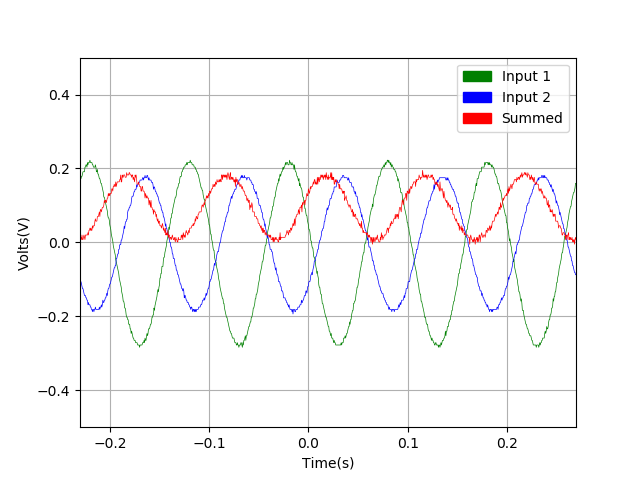
\includegraphics[width=0.95\textwidth, height=0.20\textheight]{figures/Summing/scope_4raw.png}
  %\caption{The raw data from the oscilloscope. Inputs (V1, V2) and the Summed Signal (V0)}
 \label{fig:sum_4_og_data}
\end{subfigure}\hfill
\begin{subfigure}[t]{.475\textwidth}
  \centering
  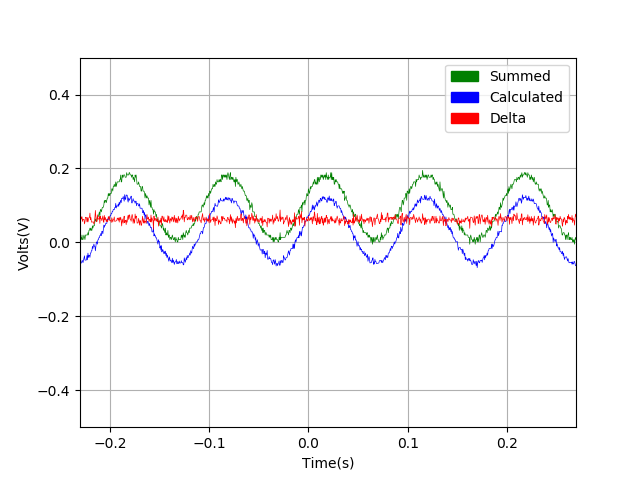
\includegraphics[width=0.95\textwidth, height=0.20\textheight]{figures/Summing/scope_4.png}
  %\caption{The summed raw data (V), calculated signal -($v_1 + v_2$)\& difference between them (delta).}
\label{fig:sum_4_calc_data}
\end{subfigure}
\caption{Sine waves Summed with 180$^\circ$ phase difference, 10Hz signal}
\end{figure}

\begin{figure}[h!]
\centering
\begin{subfigure}[t]{.475\textwidth}
  \centering
  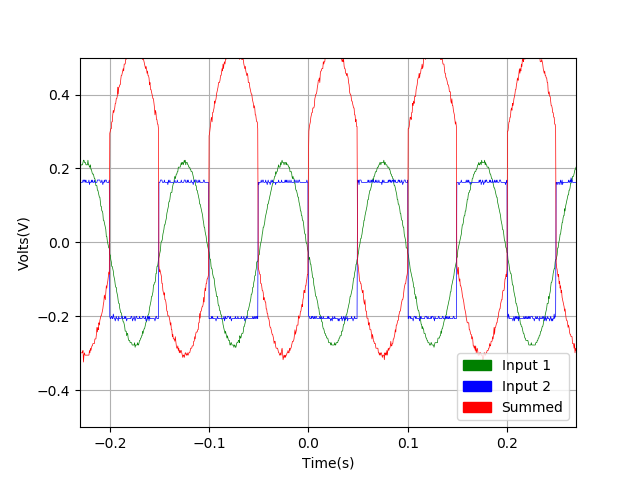
\includegraphics[width=0.95\textwidth, height=0.20\textheight]{figures/Summing/scope_6raw.png}
  %\caption{The raw data from the oscilloscope. Inputs (V1, V2) and the Summed Signal (V0)}
 \label{fig:sum_6_og_data}
\end{subfigure}\hfill
\begin{subfigure}[t]{.475\textwidth}
  \centering
  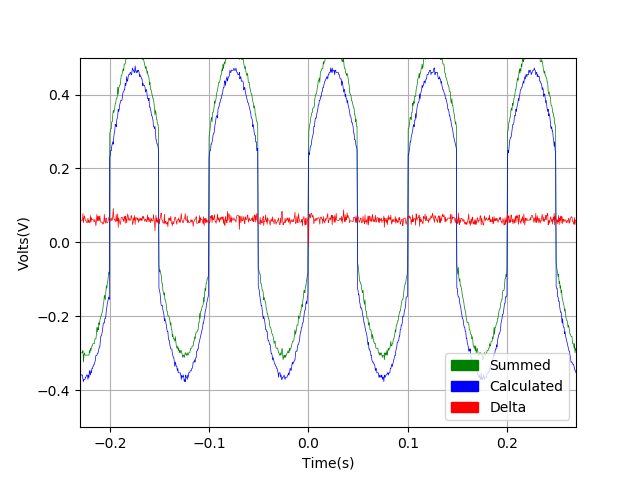
\includegraphics[width=0.95\textwidth, height=0.20\textheight]{figures/Summing/scope_6.png}
  %\caption{The summed raw data (V), calculated signal -($v_1 + v_2$)\& difference between them (delta).}
\label{fig:sum_6_calc_data}
\end{subfigure}
\caption{Sine wave summed with a square wave, 10Hz signal}
\end{figure}

\begin{figure}[h!]
\centering
\begin{subfigure}[t]{.475\textwidth}
  \centering
  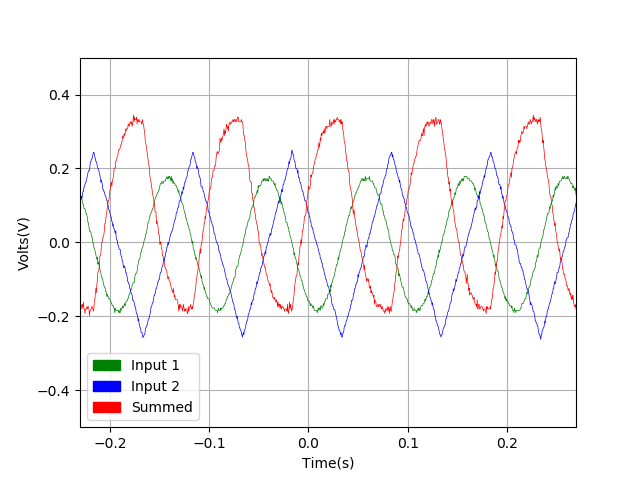
\includegraphics[width=0.95\textwidth, height=0.20\textheight]{figures/Summing/scope_8raw.png}
  \caption{The raw data from the oscilloscope. Inputs (V1, V2) and the Summed Signal (V0)}
 \label{fig:sum_8_og_data}
\end{subfigure}\hfill
\begin{subfigure}[t]{.475\textwidth}
  \centering
  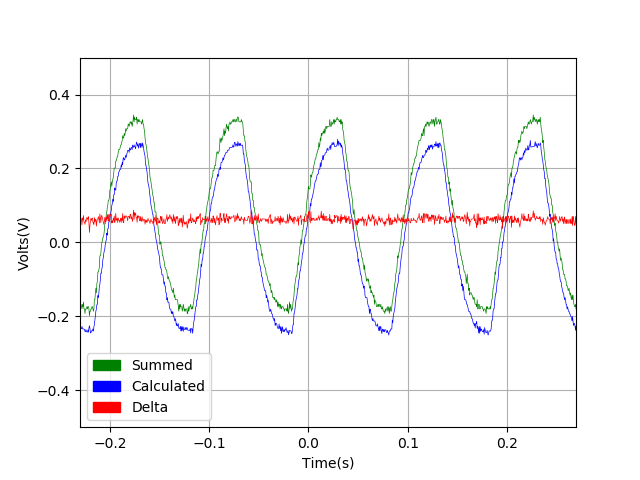
\includegraphics[width=0.95\textwidth, height=0.20\textheight]{figures/Summing/scope_8.png}
  \caption{The summed raw data (V), calculated signal -($v_1 + v_2$)\& difference between them (delta).}
\label{fig:sum_8_calc_data}
\end{subfigure}
\caption{Sine summed with a triangular, 10Hz signal, off by $\sim1/4$ a wave}
\end{figure}

\begin{figure}[h!]
\centering
\begin{subfigure}[t]{.475\textwidth}
  \centering
  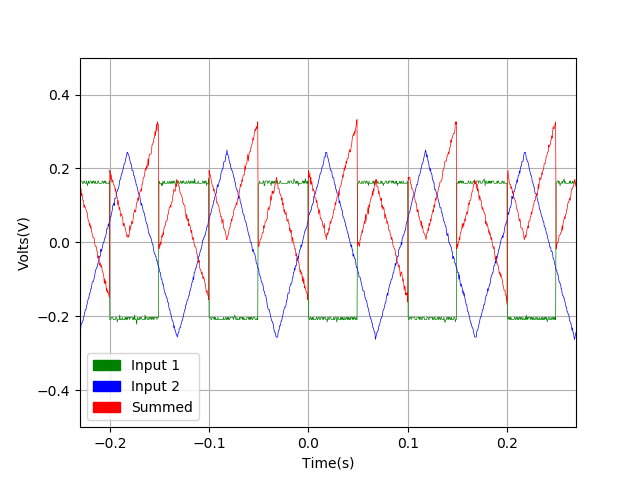
\includegraphics[width=0.95\textwidth, height=0.20\textheight]{figures/Summing/scope_10raw.png}
  %\caption{The raw data from the oscilloscope. Inputs (V1, V2) and the Summed Signal (V0)}
 \label{fig:sum_10_og_data}
\end{subfigure}\hfill
\begin{subfigure}[t]{.475\textwidth}
  \centering
  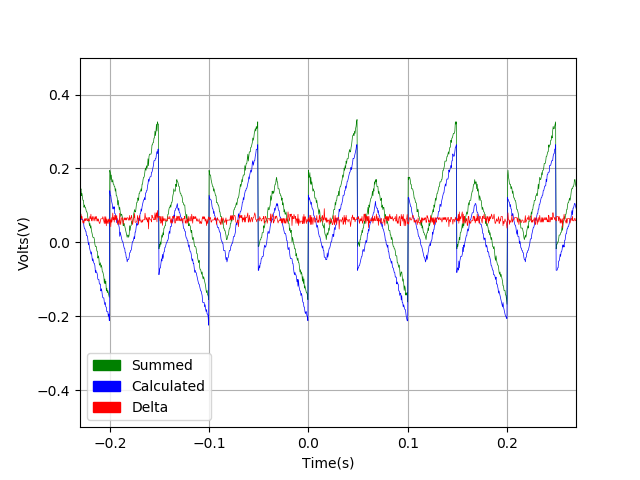
\includegraphics[width=0.95\textwidth, height=0.20\textheight]{figures/Summing/scope_10.png}
  %\caption{The summed raw data (V), calculated signal -($v_1 + v_2$)\& difference between them (delta).}
\label{fig:sum_10_calc_data}
\end{subfigure}
\caption{Square summed with a triangular, 10Hz signal off phase by $\sim1/4$ wave}
\end{figure}

\clearpage

\section{Differentiation} \label{append:diff}

Here we will present the results of the DC vs AC coupling

\begin{figure}[h!]
\centering
\begin{subfigure}[t]{.475\textwidth}
  \centering
  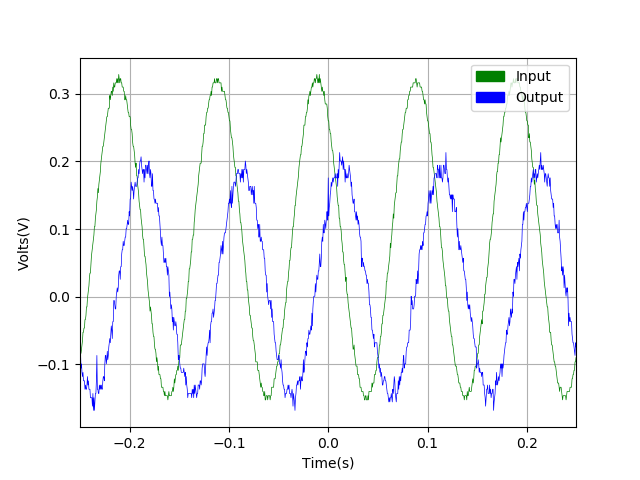
\includegraphics[width=0.95\textwidth, height=0.20\textheight]{figures/Differentiation/scope_20raw.png}
  \caption{The raw data input and output of the scope}
 \label{fig:diff_DC_raw}
\end{subfigure}\hfill
\begin{subfigure}[t]{.475\textwidth}
  \centering
  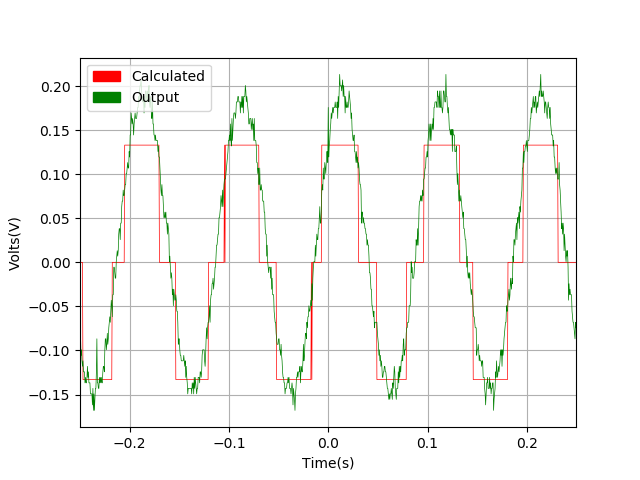
\includegraphics[width=0.95\textwidth, height=0.20\textheight]{figures/Differentiation/scope_20_calc_behind.png}
  \caption{The numerical differentiation compared with the output signal.}
\label{fig:diff_DC_filter}
\end{subfigure}
\caption{DC coupled with DC offset.}
\label{fig:diff_DC}
\end{figure}


\begin{figure}[h!]
\centering
\begin{subfigure}[t]{.475\textwidth}
  \centering
  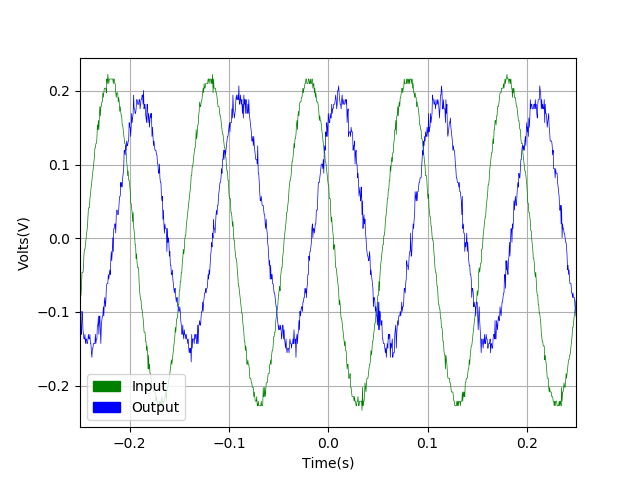
\includegraphics[width=0.95\textwidth, height=0.20\textheight]{figures/Differentiation/scope_21raw.png}
  \caption{The raw data input and output of the scope}
 \label{fig:diff_DC_raw}
\end{subfigure}\hfill
\begin{subfigure}[t]{.475\textwidth}
  \centering
  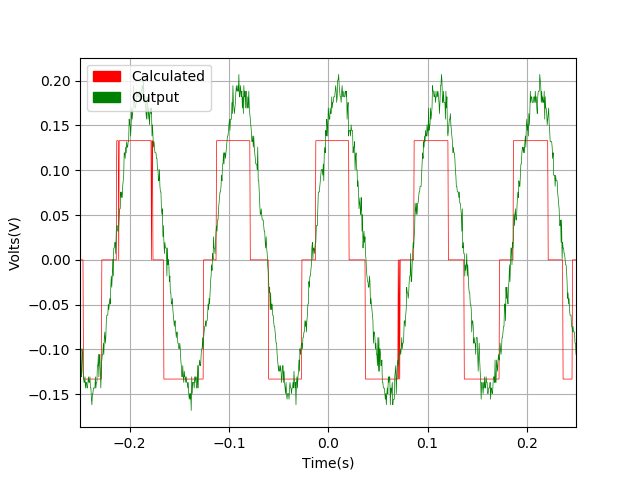
\includegraphics[width=0.95\textwidth, height=0.20\textheight]{figures/Differentiation/scope_21_calc_behind.png}
  \caption{The numerical differentiation compared with the output signal.}
\label{fig:diff_DC_filter}
\end{subfigure}
\caption{AC coupled with DC offset.}
\label{fig:diff_AC}
\end{figure}

\clearpage
\section{Forced Damped Harmonic Motion} \label{append:FDHO}

Here we will present the other results not shown in Section \ref{sec:FDHO}. 

\begin{figure}[h!]
\centering
\begin{subfigure}[t]{.475\textwidth}
  \centering
  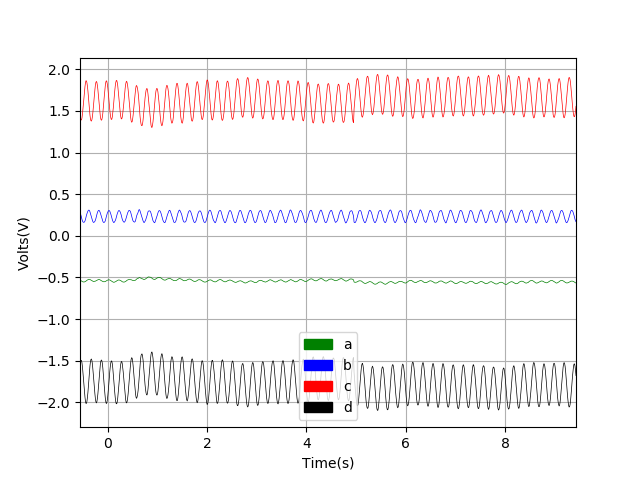
\includegraphics[width=0.95\textwidth, height=0.20\textheight]{figures/FDHO/scope_38raw.png}
  \caption{The raw data from the oscilloscope showing a,b,c,d as in Section \ref{sec:DHO}.}
 \label{fig:FDHO_5Hz_raw}
\end{subfigure}\hfill
\begin{subfigure}[t]{.475\textwidth}
  \centering
  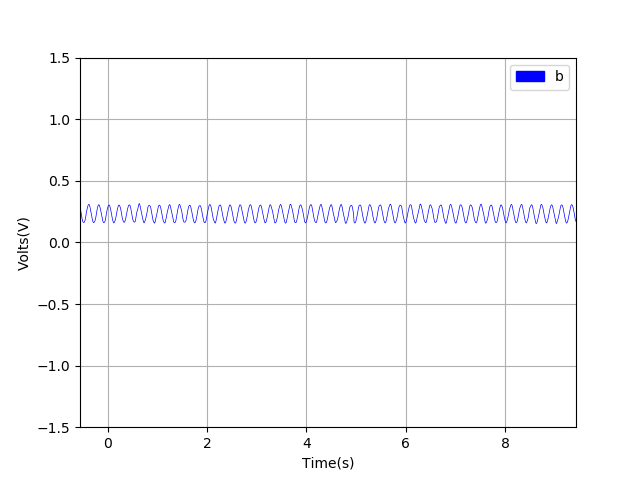
\includegraphics[width=0.95\textwidth, height=0.20\textheight]{figures/FDHO/scope_38v_2.png}
  \caption{The b output from the oscilloscope used to calculate the amplitude.}
\label{fig:FDHO_5Hz_b}
\end{subfigure}
\caption{The forced damped harmonic signal seen at 5Hz.}
\label{fig:FDHO_5Hz}
\end{figure}

\begin{figure}[h!]
\centering
\begin{subfigure}[t]{.475\textwidth}
  \centering
  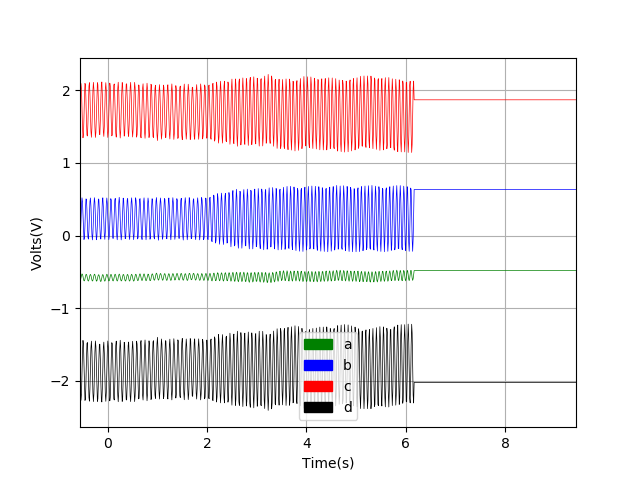
\includegraphics[width=0.95\textwidth, height=0.20\textheight]{figures/FDHO/scope_41raw.png}
  \caption{The raw data from the oscilloscope showing a,b,c,d as in Section \ref{sec:DHO}.}
 \label{fig:FDHO_14Hz_raw}
\end{subfigure}\hfill
\begin{subfigure}[t]{.475\textwidth}
  \centering
  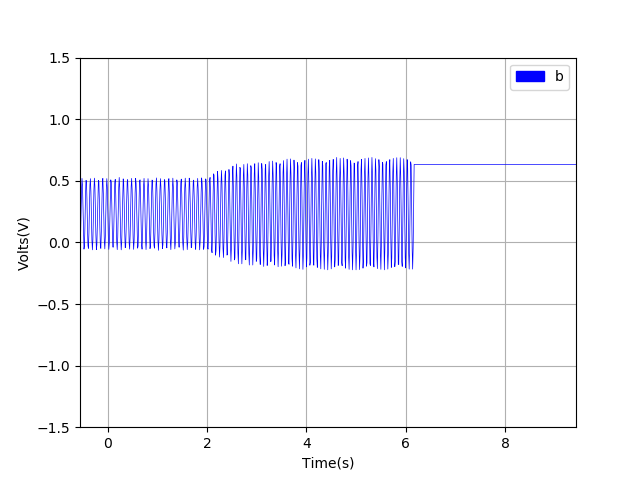
\includegraphics[width=0.95\textwidth, height=0.20\textheight]{figures/FDHO/scope_41v_2.png}
  \caption{The b output from the oscilloscope used to calculate the amplitude.}
\label{fig:FDHO_14Hz_b}
\end{subfigure}
\caption{The forced damped harmonic signal seen at 14Hz.}
\label{fig:FDHO_14Hz}
\end{figure}

\begin{figure}[h!]
\centering
\begin{subfigure}[t]{.475\textwidth}
  \centering
  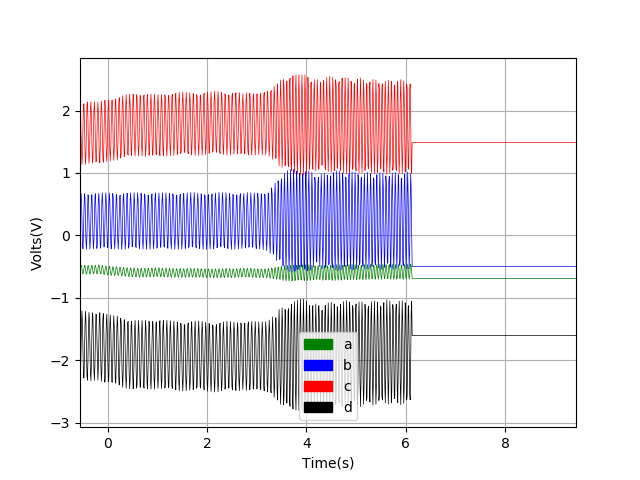
\includegraphics[width=0.95\textwidth, height=0.20\textheight]{figures/FDHO/scope_42raw.png}
  \caption{The raw data from the oscilloscope showing a,b,c,d as in Section \ref{sec:DHO}.}
 \label{fig:FDHO_16Hz_raw}
\end{subfigure}\hfill
\begin{subfigure}[t]{.475\textwidth}
  \centering
  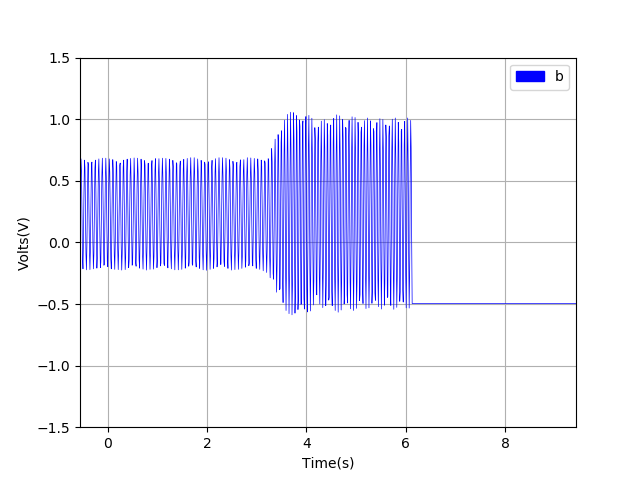
\includegraphics[width=0.95\textwidth, height=0.20\textheight]{figures/FDHO/scope_42v_2.png}
  \caption{The b output from the oscilloscope used to calculate the amplitude.}
\label{fig:FDHO_16Hz_b}
\end{subfigure}
\caption{The forced damped harmonic signal seen at 16Hz.}
\label{fig:FDHO_16Hz}
\end{figure}

\begin{figure}[h!]
\centering
\begin{subfigure}[t]{.475\textwidth}
  \centering
  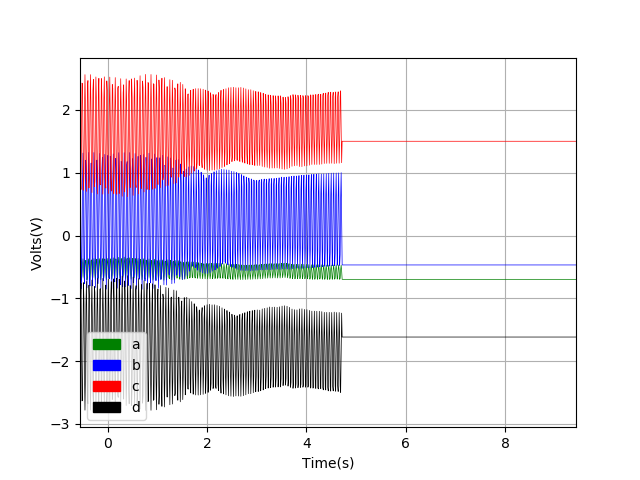
\includegraphics[width=0.95\textwidth, height=0.20\textheight]{figures/FDHO/scope_44raw.png}
  \caption{The raw data from the oscilloscope showing a,b,c,d as in Section \ref{sec:DHO}.}
 \label{fig:FDHO_20Hz_raw}
\end{subfigure}\hfill
\begin{subfigure}[t]{.475\textwidth}
  \centering
  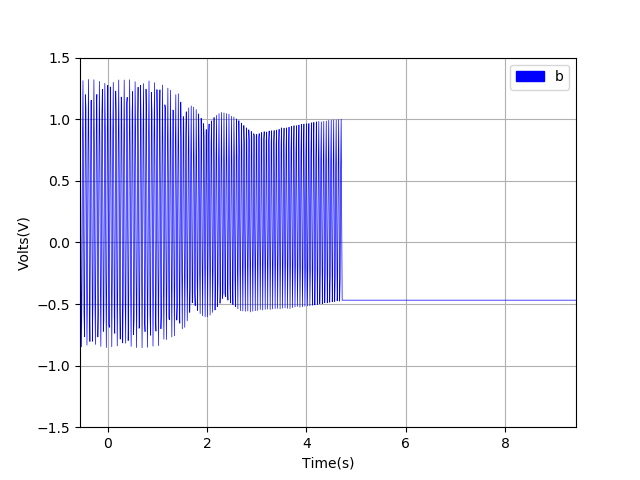
\includegraphics[width=0.95\textwidth, height=0.20\textheight]{figures/FDHO/scope_44v_2.png}
  \caption{The b output from the oscilloscope used to calculate the amplitude.}
\label{fig:FDHO_20Hz_b}
\end{subfigure}
\caption{The forced damped harmonic signal seen at 20Hz.}
\label{fig:FDHO_20Hz}
\end{figure}

\begin{figure}[h!]
\centering
\begin{subfigure}[t]{.475\textwidth}
  \centering
  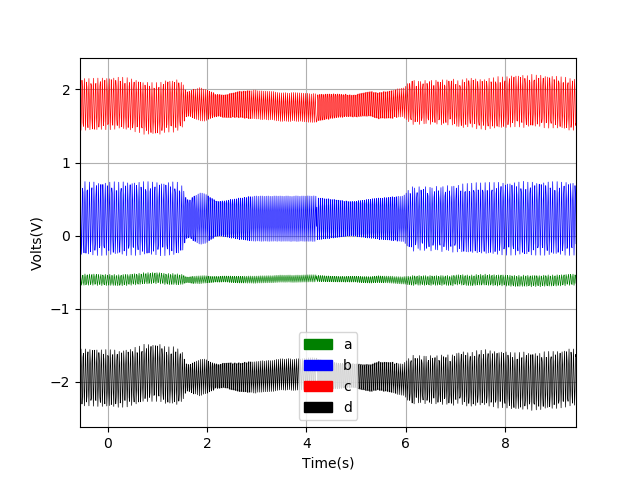
\includegraphics[width=0.95\textwidth, height=0.20\textheight]{figures/FDHO/scope_45raw.png}
  \caption{The raw data from the oscilloscope showing a,b,c,d as in Section \ref{sec:DHO}.}
 \label{fig:FDHO_25Hz_raw}
\end{subfigure}\hfill
\begin{subfigure}[t]{.475\textwidth}
  \centering
  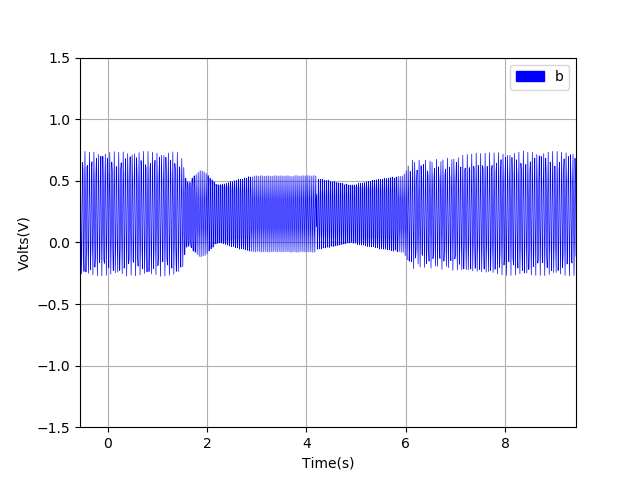
\includegraphics[width=0.95\textwidth, height=0.20\textheight]{figures/FDHO/scope_45v_2.png}
  \caption{The b output from the oscilloscope used to calculate the amplitude.}
\label{fig:FDHO_25Hz_b}
\end{subfigure}
\caption{The forced damped harmonic signal seen at 25Hz.}
\label{fig:FDHO_25Hz}
\end{figure}

\begin{figure}[h!]
\centering
\begin{subfigure}[t]{.475\textwidth}
  \centering
  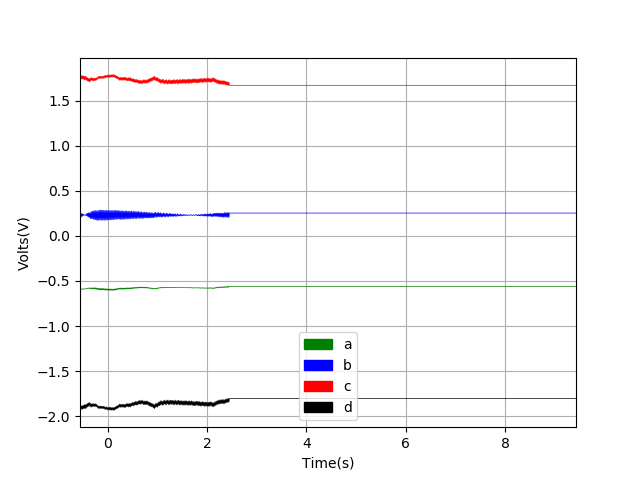
\includegraphics[width=0.95\textwidth, height=0.20\textheight]{figures/FDHO/scope_46raw.png}
  \caption{The raw data from the oscilloscope showing a,b,c,d as in Section \ref{sec:DHO}.}
 \label{fig:FDHO_50Hz_raw}
\end{subfigure}\hfill
\begin{subfigure}[t]{.475\textwidth}
  \centering
  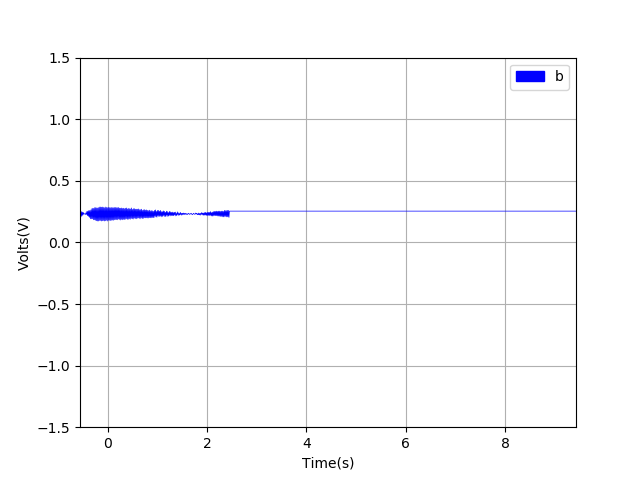
\includegraphics[width=0.95\textwidth, height=0.20\textheight]{figures/FDHO/scope_46v_2.png}
  \caption{The b output from the oscilloscope used to calculate the amplitude.}
\label{fig:FDHO_50Hz_b}
\end{subfigure}
\caption{The forced damped harmonic signal seen at 50Hz.}
\label{fig:FDHO_50Hz}
\end{figure}